
\section{Background \& Data} \label{Data}

\subsection{Natural Disasters in the United States}

Natural disasters cause numerous fatalities and billions of dollars of infrastructure damage in the United States each year \citep{Boustan_2020}. With more greenhouse gas in the atmosphere the number and severity of such disasters will increase \citep{IPCC_2021}. Table \ref{DisasterCount} shows the number of county-level disaster per year. However, note that a single disaster that affects multiple counties counts as multiple county-level disasters.

\begin{figure}[!h]
	\centering
	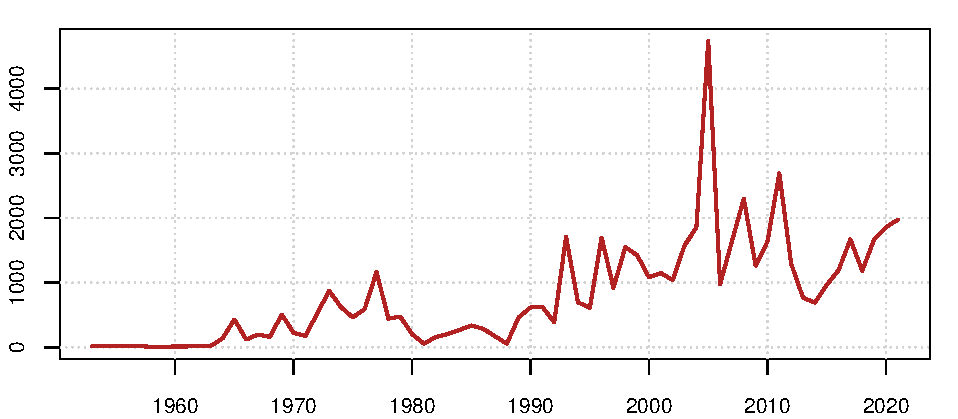
\includegraphics[scale=1]{"../Code & Data/DisasterCount.pdf"}
	\caption{Number of caounty-level natural disasters by year}
	\label{DisasterCount}
\end{figure}


Natural disasters are declared as such by the president, usually upon request by the affected state's governor. Once a disaster is federally declared, states or local governments can receive federal assistance. The Federal Emergency Management Agency (FEMA) provides data on all federally declared natural disasters, beginning in 1953. The data is easily accessible via their API \citep{rfema}. Figure \ref{DisasterMap} shows the number of declared disasters between 2009 and 2018 across the US. Table \ref{DisasterTypes} shows the types of disasters and their proportion in the FEMA data. Storms make up the largest share of disaster events. Fire and floods also form a substantial part.

\begin{figure}[!h]
	\centering
	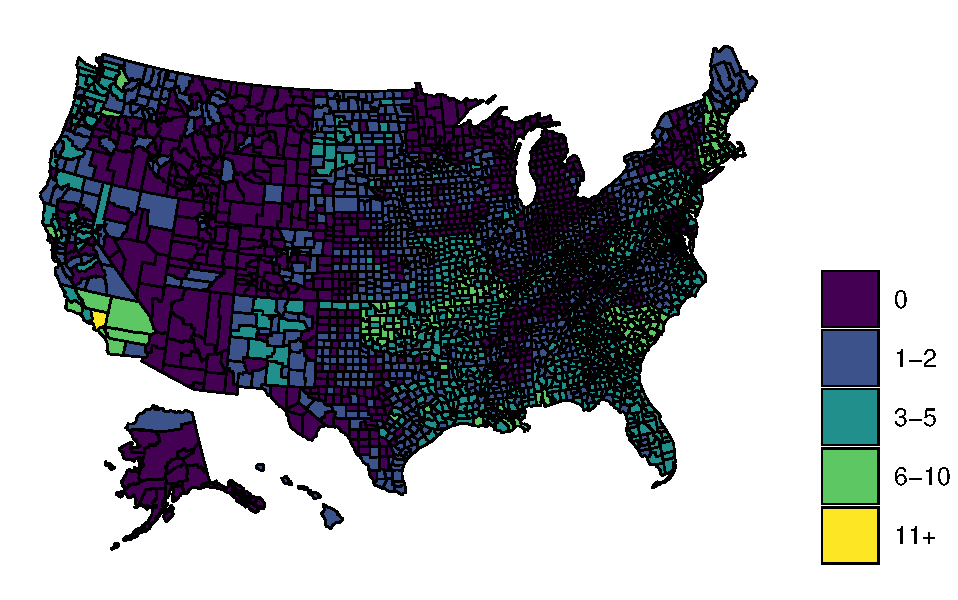
\includegraphics[scale=1]{"../Code & Data/DisasterMap.pdf"}
	\caption{Number of declared natural disasters from 2009 to 2018}
	\label{DisasterMap}
\end{figure}

\begin{table}[!h] \centering \caption{Disasters from 2009 to 2018 by type}\label{DisasterTypes}
\begin{tabular}{lrr}
\hline
\hline
Variable & N & Percent \\ 
\hline
Disaster Type & 13230 &  \\ 
... Chemical & 9 & 0.1\% \\ 
... Coastal Storm & 12 & 0.1\% \\ 
... Dam/Levee Break & 3 & 0\% \\ 
... Earthquake & 19 & 0.1\% \\ 
... Fire & 886 & 6.7\% \\ 
... Flood & 2006 & 15.2\% \\ 
... Freezing & 1 & 0\% \\ 
... Hurricane & 3094 & 23.4\% \\ 
... Mud/Landslide & 28 & 0.2\% \\ 
... Other & 7 & 0.1\% \\ 
... Severe Ice Storm & 803 & 6.1\% \\ 
... Severe Storm(s) & 5644 & 42.7\% \\ 
... Snow & 577 & 4.4\% \\ 
... Terrorist & 4 & 0\% \\ 
... Tornado & 114 & 0.9\% \\ 
... Toxic Substances & 1 & 0\% \\ 
... Tsunami & 9 & 0.1\% \\ 
... Typhoon & 11 & 0.1\% \\ 
... Volcano & 2 & 0\%\\ 
\hline
\hline
\end{tabular}
\end{table}




Nevertheless, we repeat the analysis on a second disaster dataset from an alternative source as a robustness check. The National Weather Service (NWS) provides data on storm events. In particular, this covers hurricanes, mainly affecting southern coastal regions, tornadoes, and other severe storms. These make up a very large part of all natural disasters experienced in the United States (see table \ref{DisasterTypes}). Combined they account for more than 80\% of all disaster damage in the FEMA Public Assistance Applicants Program Deliveries database.

\begin{figure}[!h]
	\centering
	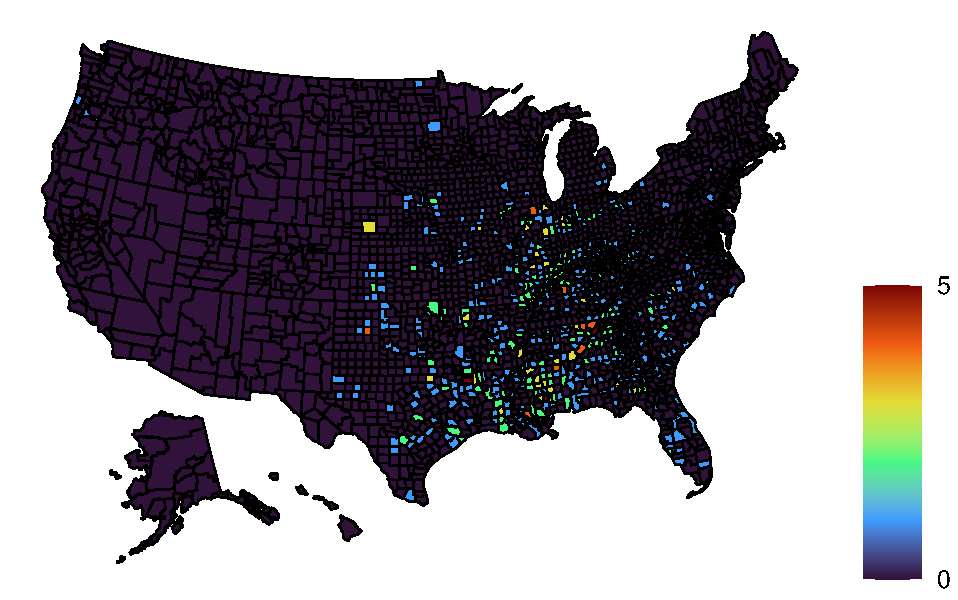
\includegraphics[scale=1]{"../Code & Data/StormMap.pdf"}
	\caption{Number of storms from 2009 to 2018}
	\label{StormMap}
\end{figure}

We only consider severe storms which are likely to cause substantial damage. Tornadoes can be classified based on estimated peak wind speeds on the Enhanced Fujita (EF) scale \citep[for more details see][]{EF_Scale}. Tornadoes with an EF scale of 0 or 1 (wind speeds of up to 110 mph) are characterized as weak. Therefore, we exclude those and only keep tornadoes with an EF scale of at least 2 (wind speeds of at least 111 mph). Unfortunately, the hurricane data does not include a similar measure, but it does include an estimated amount of property damage. We exclude all hurricanes with an estimated property damage of zero.  Storm exposure by county is shown in figure \ref{StormMap}.


\subsection{Standardized Testing Data}

Data on academic achievement is available from the Stanford Education Data Archive \citep{SEDA}. They provide mean test results from standardized tests by county, year, grade and subject among all students and various subgroups (including race, gender, and economically disadvantaged). The most recent version 4.1 covers grades 3 through 8 in mathematics and Reading Language Arts (RLA)\footnote{RLA assesses students' ability to understand what they read and to write clearly.} over the 2008-09 through 2017-18 school years.

Test scores are cohort-standardized, meaning they can be interpreted relatively to an average national reference cohort in the same grade. This makes the dataset very attractive, as test scores are nationally comparable. For instance, a county mean of 0.5 indicates that the average student in the county scored approximately one half of a standard deviation higher than the average national student in the same grade.

In addition to overall mean test scores, the data includes mean test scores for various subgroups, e.g. by ethnicity. In particular, we consider mean test scores for black, hispanic, female, and economically disadvantaged students to investiagte whether the effects differ by ethnicity, gender, or socioeconomic position. These are only reported if the subgroups' sample sizes are large enough. Thus, the number of observations for some of them is substantially smaller.

The outcomes of interest are overall mean test scores by county, and mean test scores for black, hispanic, female, and economically disadvantaged students. Figure \ref{DepVarsBoxplot} shows boxplots for the five outcomes of interest. All five mean test scores are measured on the cohort standardized scale, that is a given observation measures the distance in standard deviations from the national reference cohort. 

\begin{figure}[!h]
	\centering
	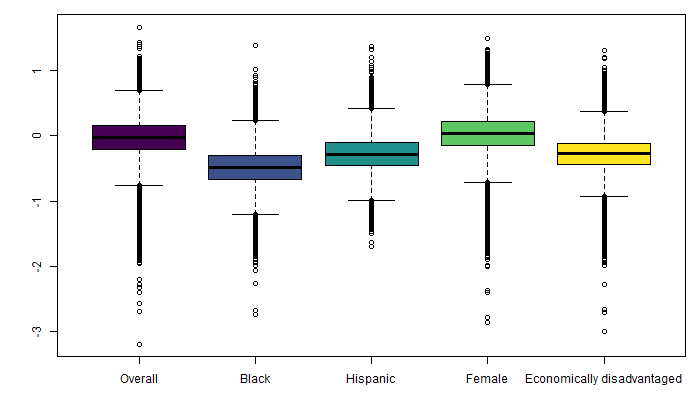
\includegraphics[scale=1]{"../Code & Data/DepVarsBoxplot.pdf"}
	\caption{Boxplots of the outcomes of interest}
	\label{DepVarsBoxplot}
\end{figure}

Due to the way the scale is constructed, overall test scores are distributed symmetrically around zero, except for a few outliers. The mean scores for black, hispanic, and economically disadvantaged students are shifted downwards by -0.48, -0.281, and -0.283 standard deviations respectively. Female mean scores are slightly above overall mean scores, meaning that female students perform slightly better than male students on average.

Furthermore, the Stanford Education Data Archive maintains a large set of covariates for each county and year. They include variables like the county's median income, unemployment and poverty rate.

Natural disasters should only have an effect on test scores if they occur before the test. Standardized tests are generally administered during spring. We will use March 1st as a cut-off point. Thus, any disaster happening within the same school year before the 1st of March will be considered. School years tend to start in late August or early September with some variation across states. We will use September 1st, meaning any disaster happening between September 1st and March 1st will be counted for a given school year. Disasters occuring in the summer or in the spring after the exams should have much less influence on performance. Thus, we do not consider disasters that occur between March 1st and September 1st.

Each disaster is assigned to a school year as described above. Then, disaster and test score data can be merged by school year and county. This yields a panel data set with six grades and two subjects for each county-year combination.


\subsection{Assistance Applications}


FEMA also provides a dataset on  their Public Assistance Applicants Program Deliveries. This contains information on applicants and their recovery priorities, including the amount of damage caused and amount of federal disaster assistance granted. Unfortunately, this data is only available starting in October 2016. Figure \ref{AssistanceMap} shows the total federal assistance awarded to counties.

\begin{figure}[!h]
	\centering
	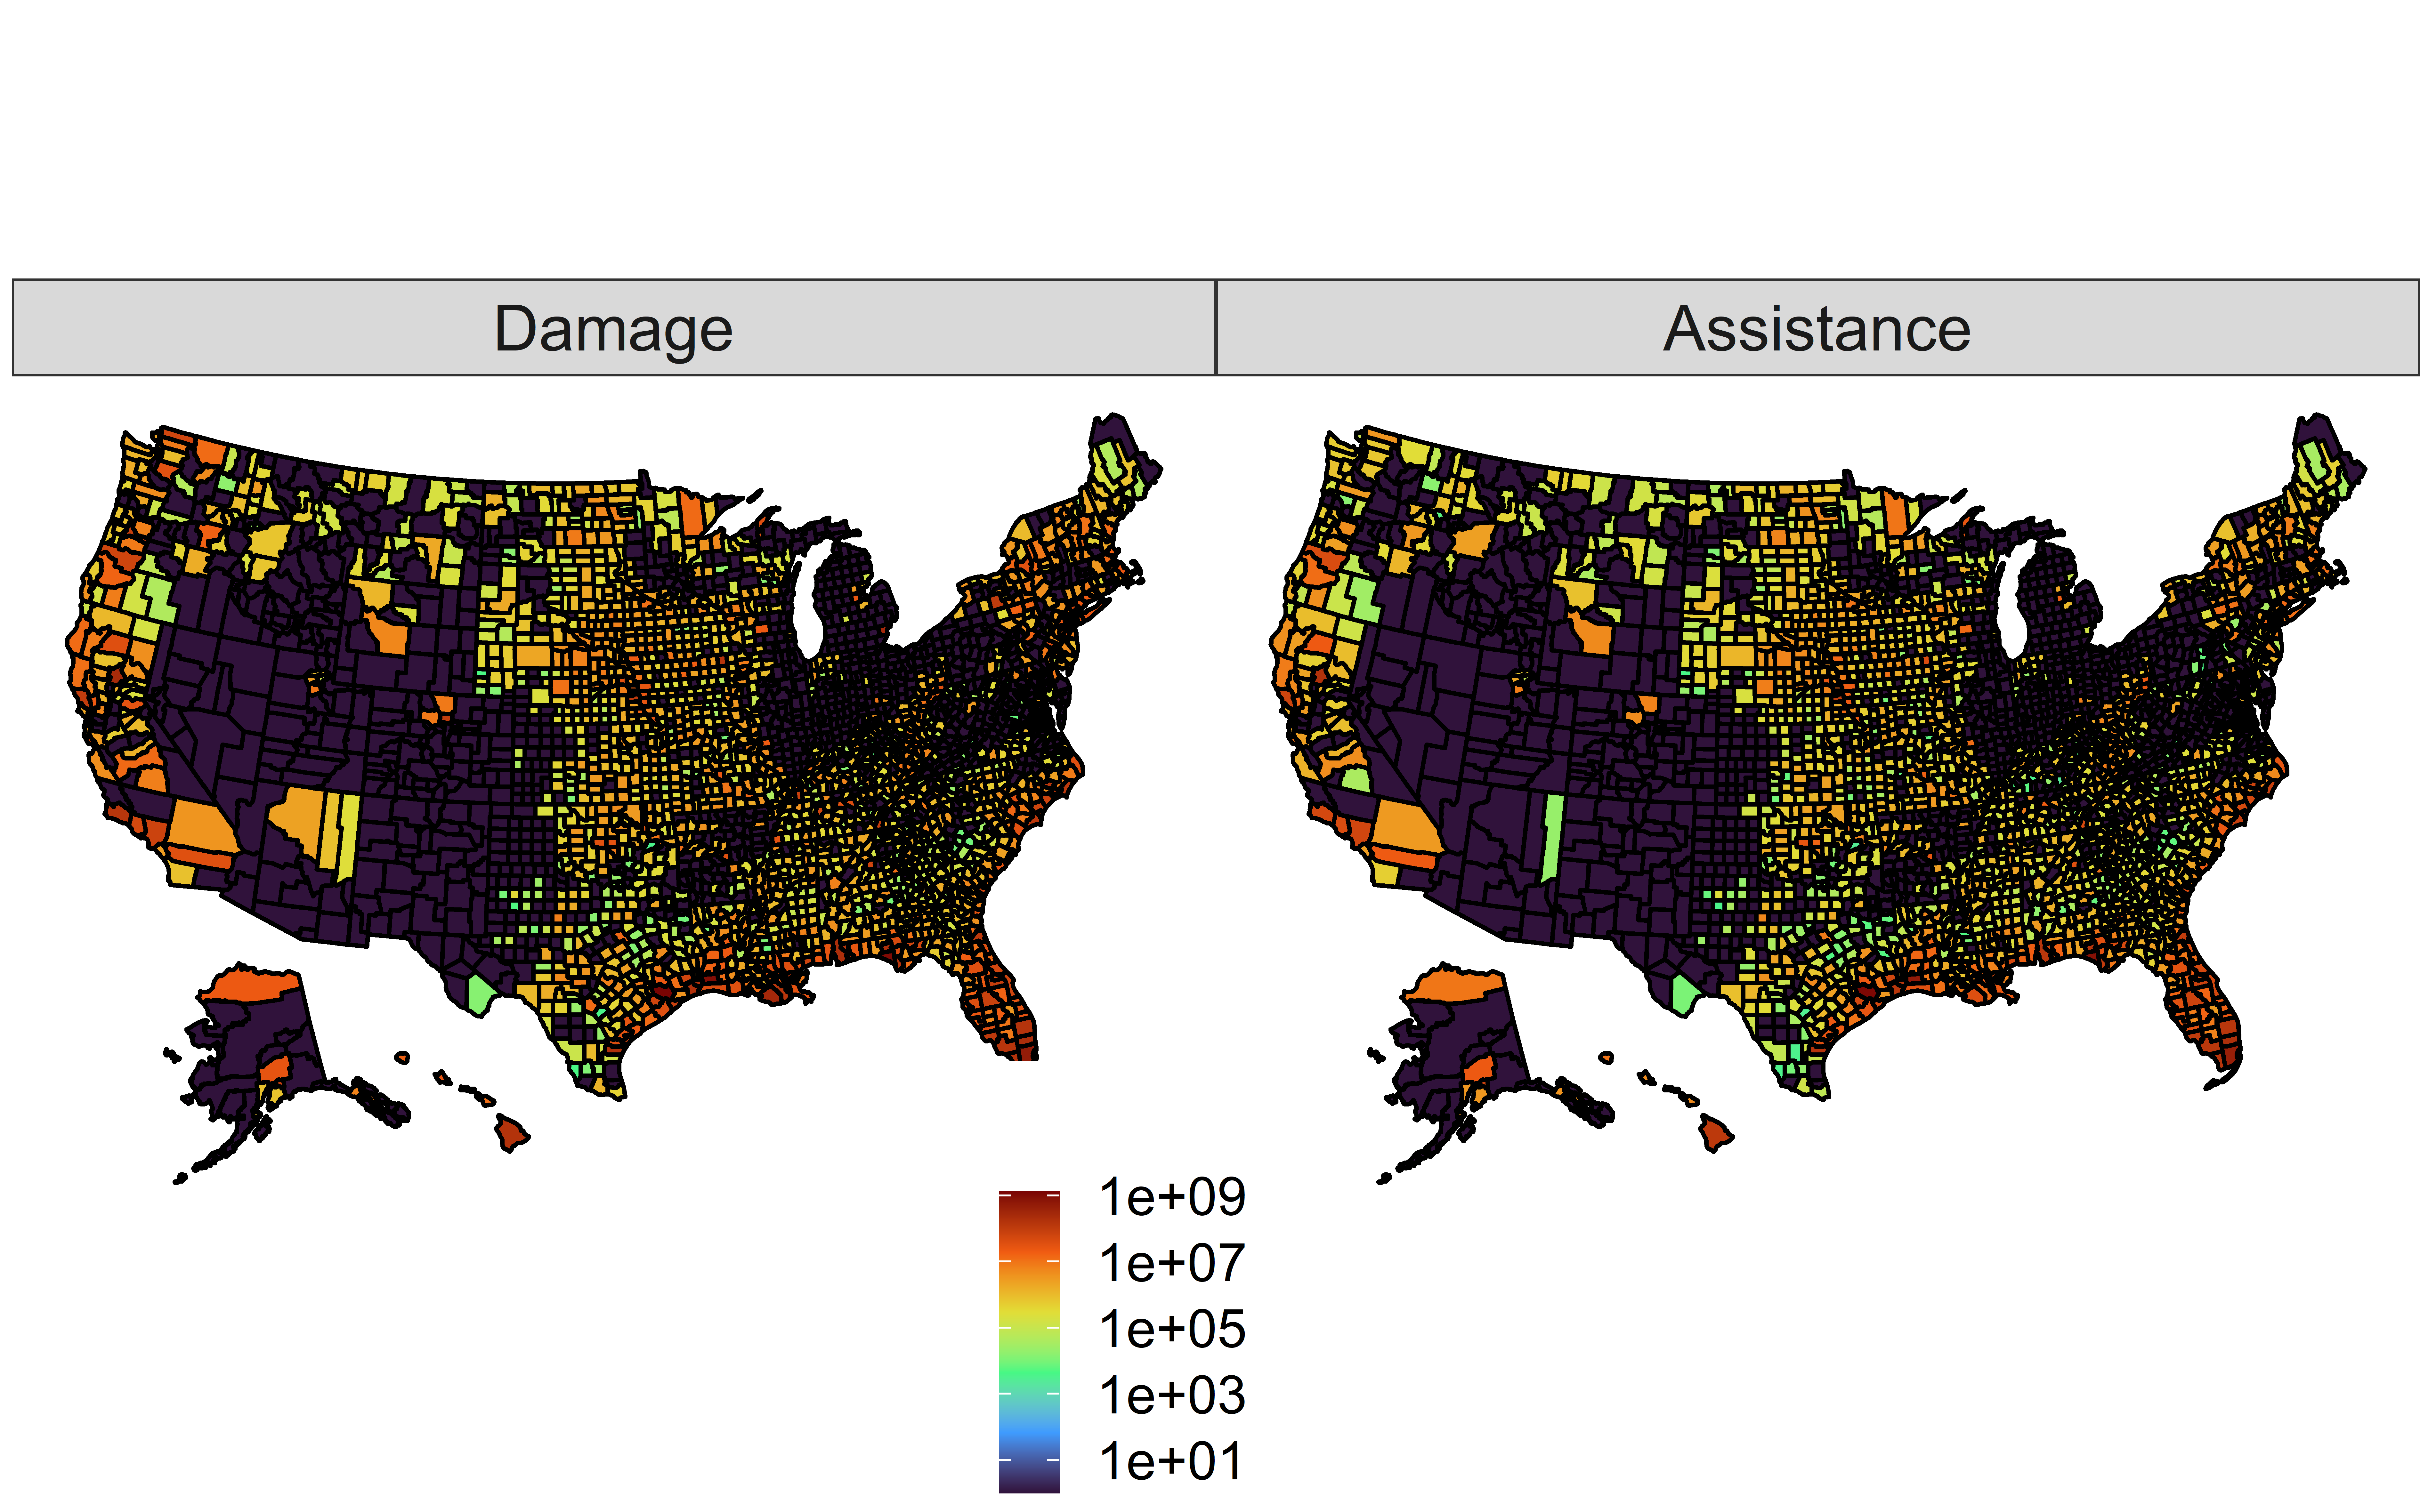
\includegraphics[scale=1]{"../Code & Data/AssistanceMap.pdf"}
	\caption{Amount of disaster damage reported by and federal disaster assistance awarded to counties since October 2016 (both in USD)}
	\label{AssistanceMap}
\end{figure}

Based on the temporal overlap between this dataset and our main dataset, that is schoolyears 2016/2017 and 2017/2018, it is possible to analyze whether counties that are affected by disasters receive federal assistance. This can be done by checking whether a county that experienced a disaster in 2016/2017 or 2017/2018 appears in the Public Assistance Applicants Program Deliveries database. In fact, only about 17.78\% of counties that experienced a disaster in that period did apply for federal assistance. Table \ref{tab:AppsByType} shows the number of disasters and the share of counties that applied for assistance following such a disaster by disaster type. It seems that the number varies dramatically by disaster type. While about 80\% of counties affected by a tornado applied for federal assistance, only about 10\% of counties affected by fires or floods did so.

\begin{table}

\caption{\label{tab:AppsByType}Share of counties that applied for federal assistance following a disaster by disaster type (schoolyears 2016-17 and 2017-18)}
\centering
\begin{tabular}[t]{lrr}
\toprule
  & Number of Cases & Applied for Assistance (in \%)\\
\midrule
Coastal Storm & 3 & 33.33\\
Dam/Levee Break & 3 & 0.00\\
Fire & 100 & 11.00\\
Flood & 270 & 41.85\\
Hurricane & 1217 & 23.25\\
Mud/Landslide & 22 & 50.00\\
Severe Ice Storm & 20 & 0.00\\
Severe Storm(s) & 164 & 28.66\\
Snow & 36 & 8.33\\
Tornado & 29 & 79.31\\
\addlinespace
Total & 1864 & 26.39\\
\bottomrule
\end{tabular}
\end{table}


It may be interesting to see how these counties differ from the ones that did apply. Figure \ref{AssistCovBoxplot} shows boxplots by county application status. Counties that did apply for federal disaster assistance tend to have lower median income, higher poverty rates, and higher shares of single motherhood. Thus, it seems that counties that had to apply for federal disaster assistance were more socially vulnerable in the first place. However, the direction of causality is not clear. Possibly these counties are more vulnerable to natural disasters and are also poorer or more socially vulnerable because of it. Alternatively, counties that are poorer could be more likely to apply for public disaster aid as they have fewer private resources.

\begin{figure}[!h]
	\centering
	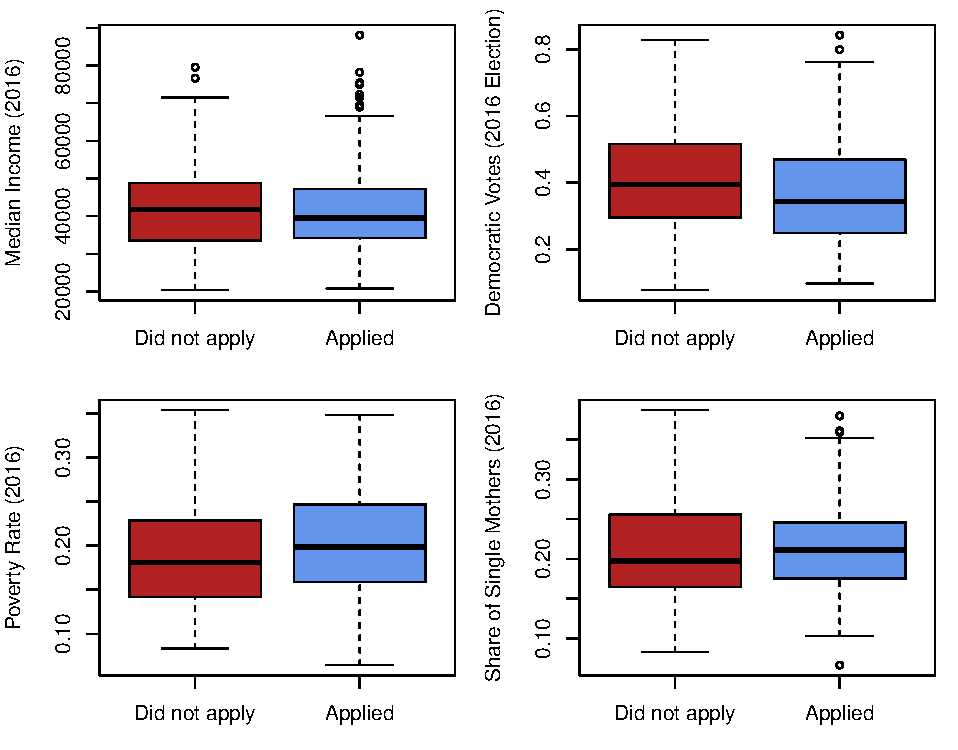
\includegraphics[scale=1]{"../Code & Data/AssistanceCovBoxplot.pdf"}
	\caption{Boxplots by application status}
	\label{AssistCovBoxplot}
\end{figure}

It is also interesting whether variation in the federal assistance procedure may be driven by political factors. Visually, democratic votes in the 2016 election (almost coincides with the start of the Public Assistance Applicants Program Deliveries dataset) tend to be lower in counties that applied. That is, counties that applied for federal assistance tend to vote more Republican. Logistic regression results confirm the visual impression (see Appendix \ref{AppendixA}). While this is not necessarily a causal effect, it could be an indication that a Republican president may be more hesitant awarding disaster assistance to Democratic counties.


